\documentclass{article}

\usepackage{times}
\usepackage{graphicx}
\usepackage{latexsym}

\usepackage{bm}
\usepackage{amsbsy}
\usepackage{amsmath}
\usepackage{amsfonts}
\usepackage{amssymb}

\usepackage{subfigure}

\usepackage{theorem}

\theoremstyle{theorem}
\newtheorem{theorem}{Theorem}

\theoremstyle{definition}
\newtheorem{definition}{Definition}
\newtheorem{remark}{Remark}

\newcommand{\bu}[1]{\mathbf{#1}}
\newcommand{\bv}[1]{\bm{#1}}


\newcommand{\X}{\mathbf{X}}
\newcommand{\Y}{\mathbf{Y}}
\newcommand{\Z}{\mathbf{Z}}
\newcommand{\x}{\mathbf{x}}
\newcommand{\y}{\mathbf{y}}
\newcommand{\z}{\mathbf{z}}
\newcommand{\argmax}[1]{\underset{#1}{\operatorname{arg}\,\operatorname{max}}\;}



\title{Practical Considerations for Testing the Cajamar Use Case}
%\author{Sigve Hovda \\
%Norwegian University of Science and Technology\\
%Department of Computer and Information Science,
%Trondheim, Norway\\
%sigveh@idi.ntnu.no}
\date{}


\begin{document}
\maketitle

There are two application scenarios here.  The first one is prediction of whether a client will default within two years or not and the second is related to the benefit of a marketing campaign. For clarity we have added the description about the data set from delivery 2.1 without any modification.

\section{Description from 2.1}

%-------------------------------------------------------------------------------------------------------
\subsection{Predicting probability of default} \label{SubSection:Predicting}
%-------------------------------------------------------------------------------------------------------

Our objective is to tackle the current limitations of the risk prediction problem by \textit{daily} learning the predictive model and also updating the risk of default for every bank customer. Dependences among the variables will now be considered, as well as including all the variables in the analysis. With these changes, Cajamar plans to improve the quality of the prediction model by increasing the area under ROC curve significantly.


Therefore, the process will consist in building a \textit{training set} as well as a set of customers to be evaluated, called \textit{evaluation set} (see Deliverable 1.2~\cite{Fer14b}). How these data sets are generated gives us some insights into the nature of this risk prediction problem (see Figure~\ref{Figure:CajaMarTimeLine} for a better understanding):

%Next, we detail how these data sets are collected .
%Figure~\ref{Figure:CajaMarTimeLine} illustrates how both evaluation and training data sets are collected within a time-line. The current time is denoted as $t$ and the time $2$ years back as $k$, i.e., $k=t-2$ years. 

\begin{figure}[ht!]
\centering
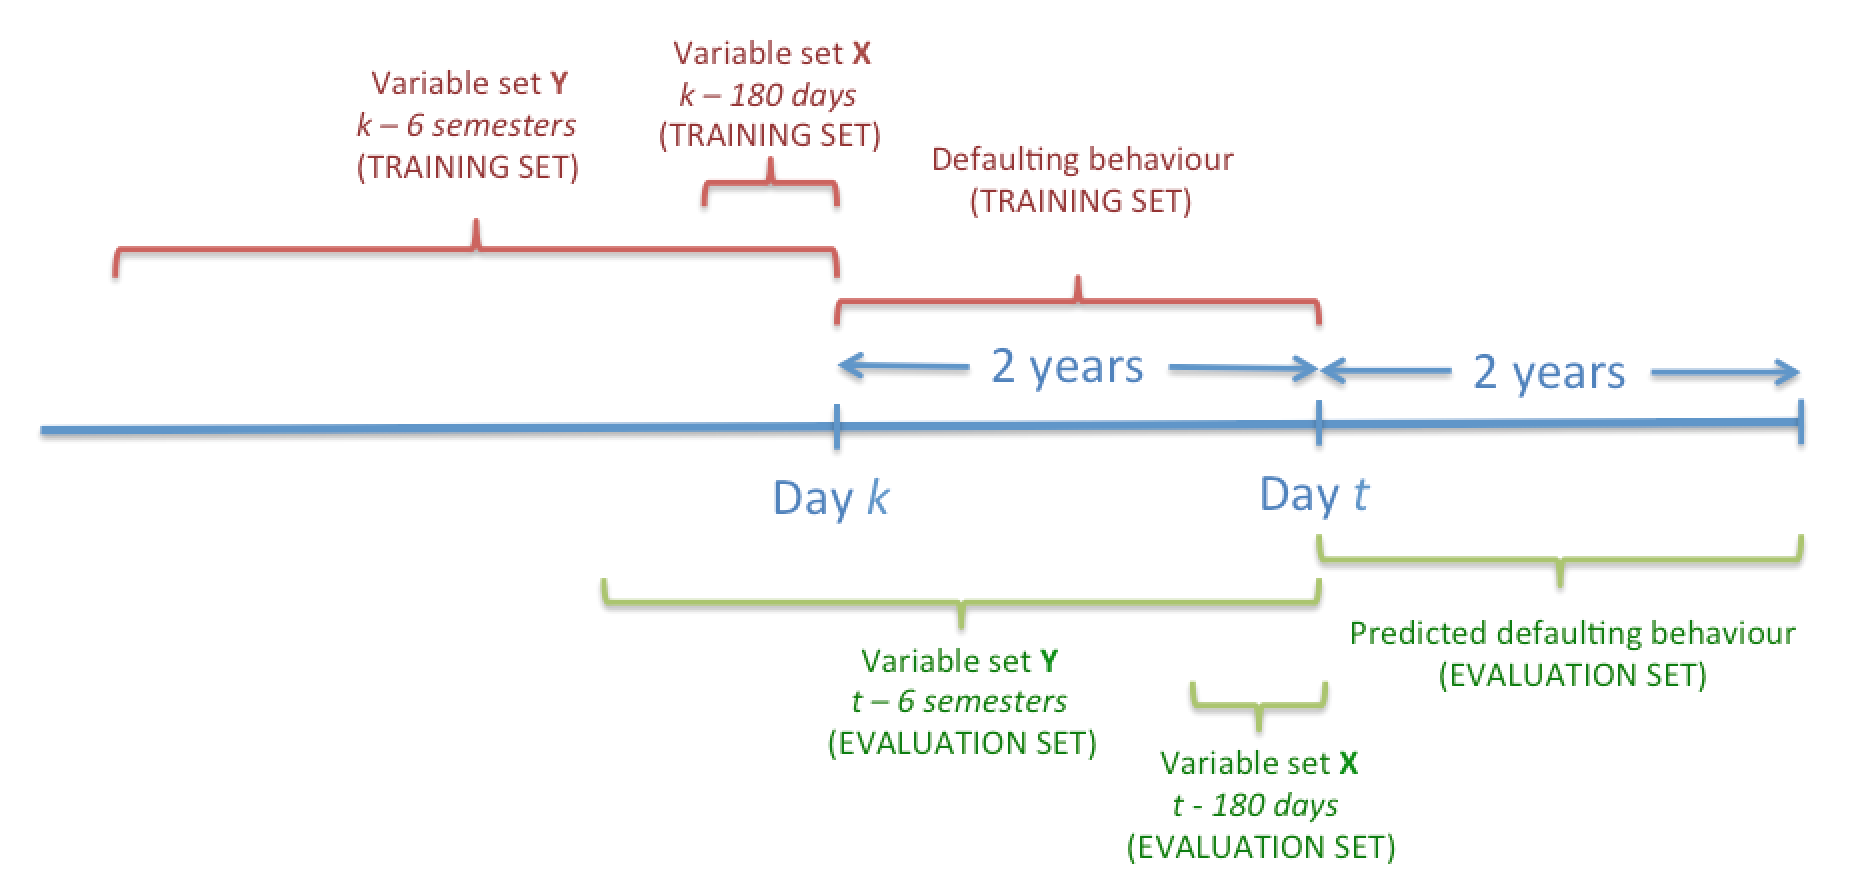
\includegraphics[scale=0.45]{figures/CajaMarTimeLine}
\caption{\label{Figure:CajaMarTimeLine}Time-line showing the generation of the evaluation (in green) and training (in red) data sets. $t$ refers to the present time and $k$ corresponds to time $t-2$\ years. Both in the training and test data sets, there are two disjoint groups of variables, denoted as $\X$ and $\Y$, with different past information considered, $180$ days back (daily) and $6$ semesters back (by semester), respectively.}

\end{figure}

\begin{itemize}

\item \textbf{Model evaluation data set:} This data is created at time $t$ and contains a record for every client to be evaluated. Note that information about the predicted defaulting behaviour is missing at time $t$ and it will be obtained after performing inference on the model. Predictive variables refer here to the financial activity and payment behaviour of the customers in recent past as well as to their socio-demographic information which usually does not change over time. 

There are attributes, denoted as $\X$, for which information during the last 180 days is considered. 
%recent \textcolor{red}{{\bf financial activity}}of a customer refers to attributes such as ``account balance'', ``number of credit card operations'', etc. stored in the last 180 days. 
These attributes usually change daily for a customer, so they are encoded by introducing a set of variables for each attribute, one for each day back from the current time $t$. Hence, the financial activity of a customer is specified by a number of variables equal to 180 times the number of attributes. For others attributes, denoted as $\Y$, we are interested in information from the last $36$ months grouped by semester. 
%In the case of \textcolor{red}{{\bf past payment behaviour}}, the attributes refer to variables related to \textcolor{red}{payments inside Cajamar (loans, mortgages, credits, etc.).} Information from the last 36 months grouped by semester is considered for these variables. 
Therefore, similar to previous group of variables, $6$ variables for each of these attributes will be considered. Finally, there are some other static variables, denoted as $\Z$, not included in Figure~\ref{Figure:CajaMarTimeLine} as they are not indexed over time. The data set for the evaluation of customers is depicted in Table~\ref{tab:EvaluationDataset}. 


%with information about \textcolor{red}{payments to other financial institutions or companies (phone and electricity bills, public bodies, etc.)} 
%are included in this group of variables. They are denoted as .

%The group of variables denoted as $\Z$ mainly includes socio-demographic variables and they are not indexed over time as they remain fixed.  

\begin{table}[ht!]
\centering
\begin{tabular}{c|ccc|ccc|c}
	&\multicolumn{3}{c|}{Days} & \multicolumn{3}{c|}{Semester} \\
     Time $t$              & $\X^{(t-180)}$ & $\ldots$ & $\X^{(t-1)} $ & $\Y^{(t-6)}$  & $\ldots$ & $\Y^{(t-1)} $ & $\Z$  \\  
\hline
Client$_1$  &                                                  &              &                     &                               &                     &        \\ 
$\vdots$      &                                                 &               &                     &                                &                     &      \\ 
Client$_n$  &                                                &               &                     &                                &                     &     \\ 
\end{tabular}
\caption{Evaluation data set at time $t$ for all the clients. Three groups of attributes $\X$, $\Y$ and $\Z$ are distinguished according to the past information required. Current time is denoted as $t$.}
\label{tab:EvaluationDataset} 
\end{table}

Thus, the objective is to compute the probability of defaulting within the following two years of each record from the evaluation data set, and afterwards update the risk table in the system (see Table~\ref{tab:riskTable}).

\begin{table}[ht!]
\centering
\begin{tabular}{c|ccc|ccc|c}
     Time $t$  & Risk of being defaulter \\  
\hline
Client$_1$  &    $r_1$  \\ 
$\vdots$      &   $\vdots$   \\ 
Client$_n$  &   $r_n$  \\ 
\end{tabular} 
\caption{Risk table for the bank customers where $r_i$ represents the probability of being defaulter for customer $i$.}
\label{tab:riskTable}
\end{table}

If, at some point, the probability of default of a customer rises above a predefined threshold, the bank may take preventive actions to reduce the risk of defaulting by this customer.


\item \textbf{Model training data set:}  This data set is also built at time $t$ in a similar way as the evaluation data. It contains the same set of features as well as the target variable \textit{Defaulter} but with information referred to time $k$ instead (two years back). Note that, at time $t$, we have information of the \textit{Defaulter} variable in the period of time from $k$ to $t$. Thus,  Defaulter$^{(k)}$ indicates if at some point in this period she/he was a defaulter.

The data set for training/updating the model is depicted in Table~\ref{tab:TrainingDataset}.
\begin{table}[ht!]
\centering
\begin{tabular}{c|ccc|ccc|c|c}
	&\multicolumn{3}{c|}{Days} & \multicolumn{3}{c|}{Semester} & \\
     Time $t$              & $\X^{(k-180)}$ & $\ldots$ & $\X^{(k-1)} $ & $\Y^{(k-6)}$  & $\ldots$ & $\Y^{(k-1)} $ & $\Z$ & Defaulter$^{(k)}$\\  
\hline
Client$_1$  &                                                  &              &                     &                               &                     &        &  \\ 
$\vdots$      &                                                 &               &                     &                                &                     &       & \\ 
Client$_n$  &                                                &               &                     &                                &                     &     & \\ 
\end{tabular} 
\caption{Training data set built at time $t$ with $k=t - 2$ years.  The notation for predictive variables is the same as in Table~\ref{tab:EvaluationDataset}.}
\label{tab:TrainingDataset} 
\end{table}

Table~\ref{tab:TrainingDataset} shows the training data set where each record contains the values for all predictive variables and a class value labelled as \emph{non-defaulter} only when there is no evidence of defaulting in the period from $k$ to $t$ (2 years). 

\end{itemize}

\section{Test and evaluation regime}

The training set above is actually the data set that we are going to train on and also test on. This may be a source to confusion, but from now on the training set above will be defined as the dataset and the evaluation set is not even considered in relation to testing. 

The only criterion for being a member of the dataset is that the member has been a client continuously from day $k$ and up to day $t$.  Every member of the dataset has a class label that is either non defaulter or defaulter.  There are no missing values related to class labels.  However, there are missing values related to attributes.  In particular, some of the clients where not clients in the whole three year period before day $k$.  Cajamar will manually fill in all relevant missing values.  Formally, every member $i$ of the dataset has a vector of explanatory variables that is denoted by $\bv{x_i} =\{ \X_i^{(k-180)},  \X_i^{(k-1)}, ...\Y_i^{(k-6)}, \Y_i^{(k-1)},\Z_i\}$.  

We will divide this data set into a training set and a test set by a completely random process.

\subsection{Requirements for the first use case scenario: default prediction}

In the first use case scenario, it is required that the AUROC should be above 0.90.
 
The Bayesian network basically computes the probability $P(\mbox{Default}_i \,|\, \bv{x_i})$ and the classification rule is
$P(\mbox{Default}_i \,|\, \bv{x_i}) \geq C$.  The ROC curve is computed by basically plotting the rate of true positives against the rate of true negatives for various choices of $C$.  AUROC is the area under the graph.  (There is also another way of computing AUROC which do not involve computing the rate of true positives and rate true negatives for various $C$, but this is omitted in this discussion.)

\subsubsection*{Questions: }
\begin{enumerate}
\item How many defaulters and non defaulters do we have on both the training set and the test set?
\item Can you go though all the information and make sure that it is correct.
\end{enumerate}


\subsection{Requirements for the second use case scenario:  AMIDST induced marketing campaign}

A marketing campaign in Cajamar involves two steps.  The first step is to find clients that have a high probability of signing what is offered (for instance a credit card).  The second step is to filter out clients that are risky in terms of defaulting.
The testing regime involves testing each step separately.

The first step is difficult to test. We suggest that the Amidst profiler finds a list of a certain number of clients that are manually inspected by the marketing department in Cajamar. This list can for instance be compared to a list of clients with high contracting probability from a former campaign.

There are more opportunities with testing the second step.  After performing step one the test data set is reduced to a set of clients with a high contracting probability (i.e. above a certain level).  Let the clients in this data set be $(x_i, y_i)$, where $y_i$ is either default or not default and $x_i$ is a vector of explanatory variables.  It makes sense to compute AUC for both the current method and the Amidst method to compare the two methods.  This comparison will say something about the ability of the filter to take out defaulters, while keeping the non defaulters.  However, we must assume that the real probability of contracting $P(\bv{x_i})$ is completely independent of whether the client will actually default or not.

Moreover, in Delivery 1.2, it is required that the benefit of a AMIDST induced marketing campaign should be more than 5 percent higher than a normal campaign.  In order to discuss such a requirement we have to iintroduce a function that describes the financial loss of a certain classification rule compared to a classification rule that make no mistakes. 

In this paper, we define the \emph{loss function} as a real and lower-bounded function $L(x_i, h(x_i), y_i)$. It takes into account the explanatory variables for each client $x_i$, the predicted class $h(x_i)$ and the true class label $y_i$. 

In the current system in Cajamar the classification rule is denoted $h_{\mbox{Current},L_1}$ and is defined by

\begin{equation}
\label{def:empRisk}
h_{\mbox{Current},L_1}(x_i) = P_{\mbox{Current}}(\mbox{Default}_i \,|\, \bv{x_i}) \leq L_1 
\end{equation}
where the probability for defaulting client $i$ are $P_{\mbox{Current}}(\mbox{Default}_i \,|\, \bv{x_i})$.  Here, $L_1$ is a chosen classification limit. 

We let the cost of excluding client $i$ that does not default as $c_i(0|1)$ and also the cost of including client $i$ that does default as $c_i(1|0)$.  Both costs are related to the size of the potential offer.  Also, we make the assumption that the real probability of contracting $P(\bv{x_i}) = p$ is completely independent of whether the client will actually default or not.  The loss function below is of interest

\begin{equation}
\label{def:empRiskBank}
L(x_i, h_{\mbox{Current},L_1,L_2}(x_i) , y_i) = 
\begin{cases}
0     &\quad \mbox{for} \quad h_{\mbox{Current},L_1,L_2}(x_i) = 0 \quad \& \quad y_i = 0\\
p c_i(1|0)    &\quad \mbox{for} \quad h_{\mbox{Current},L_1,L_2}(x_i) = 1 \quad \& \quad y_i = 0\\
p c_i(0|1)      &\quad \mbox{for} \quad h_{\mbox{Current},L_1,L_2}(x_i) = 0 \quad \& \quad y_i = 1\\
0   &\quad \mbox{for} \quad h_{\mbox{Current},L_1,L_2}(x_i) = 1 \quad \& \quad y_i = 1.
\end{cases}
\end{equation}
Notice that $L$ is an array of $n \times 2\times 2$ elements. Cajamar can estimate $c_i(0|1)$ and $c_i(1|0)$ for all clients in the database.

The empirical risk is found by averaging the loss function on the training set given by 

\begin{equation}
\label{def:empRisk}
R_{emp}(h_{\mbox{Current},L_1,L_2}, \bv{x}) = n^{-1} \sum_{i=1}^n L(x_i, h_{\mbox{Current},L_1,L_2}(x_i), y_i).
\end{equation}

It is now possible to calculate the empirical risk involved with using both the current filter and also the Amidst filter.  It is therefore possible to estimate the ratio between the costs and therefore see whether there is more than 5 percent gain in using the Amidst default filter compared to using the current default filter.  Notice that in terms of estimating this gain percentage it is not needed to estimate $p$.  However, it could be estimated from the number that accepted the offer on an old campaign.


\subsubsection*{Calculating empirical risk on an old campaign}

It is also possible to use an old campaign to test the improvement of using the Amidst default filter in addition to the current filter. 

Consider an old campaign that was done more than two years ago. Even though costs and default/non defaults are known for all clients, the loss function is only known on the clients that was targeted in that campaign.  This makes this discussion complicated. 

\begin{equation}
\begin{split}
\label{eq:amidst}
h_{\mbox{Current},L_1,L_2}(x_i) = &
P_{\mbox{Current}}(\mbox{Default}_i \,|\, \bv{x_i}) \leq L_1
 \, \& \,
P_{\mbox{Current}}(\mbox{Contract}_i \,|\, \bv{x_i}) \geq L_2.
\end{split}
\end{equation}


The empirical risk for the old campaign is not taking into account the financial loss related to excluding a number of clients that actually would have contracted and not defaulted.  Said with other words, the empirical risk is not taking into account losses related to when $h_{\mbox{Current},L_1,L_2}(x_i) = 0$, and $y_1 = 1$.  In such a calculation none of the $c_i(0|1)$s are used.  The empirical risk will therefore be less than the true risk (which would take the above point into account).

A simple test is to use the Amidst toolbox to provide an additional filter related to default prediction on top of the old classification rule.  Mathematically this is

\begin{equation}
\begin{split}
\label{eq:filter}
h_{\mbox{Amidst filter},L_1,L_2,L_3}(x_i) = &
P_{\mbox{Current}}(\mbox{Default}_i \,|\, \bv{x_i}) \leq L_1
 \, \& \,
P_{\mbox{Current}}(\mbox{Contract}_i \,|\, \bv{x_i}) \geq L_2
\, \& \,  
\\ &
P_{\mbox{Amidst filter}}(\mbox{Default}_i \,|\, \bv{x_i}) \leq L_3.
\end{split}
\end{equation}
This calculation of empirical risk is biased by the same amount as the old method.  It makes therefore sense to compare $R_{emp}(h_{\mbox{Amidst filter},L_1,L_2,L_3}, \bv{x}) $ with $R_{emp}(h_{\mbox{Current},L_1,L_2}, \bv{x}) $.
The benefit of using the Amidst model as additional filter can therefore be quantified.

It is also of interest to examine this classification rule

\begin{equation}
\begin{split}
\label{eq:amidst}
h_{\mbox{Amidst},L_1,L_2}(x_i) = &
P_{\mbox{Amidst}}(\mbox{Default}_i \,|\, \bv{x_i}) \leq L_1
 \, \& \,
P_{\mbox{Current}}(\mbox{Contract}_i \,|\, \bv{x_i}) \geq L_2.
\end{split}
\end{equation}
The challenge related to calculating $R_{emp}(h_{\mbox{Amidst},L_1,L_2}, \bv{x})$ is that the associated loss function 
$L(x_i, h_{\mbox{Amidst},L_1,L_2}(x_i) , y_i)$ is only known for clients satisfying the statement $h_{\mbox{Current},L_1,L_2}(x_i) = 1$.  

Since different clients are added in the Amidst induced campaign, $R_{emp}(h_{\mbox{Amidst},L_1,L_2}, \bv{x})$ is biased differently than $R_{emp}(h_{\mbox{Current},L_1,L_2}, \bv{x})$. This statement holds even when the classification limits are the same. 

However there is another way to compare $R_{emp}(h_{\mbox{Amidst},L_A,L_2}, \bv{x})$ and $R_{emp}(h_{\mbox{Current},L_C,L_2}, \bv{x})$, since both methods include the same rule for removing customers that will not contract, then we can make the "wild" assumption that anyone that is offered will contract.  This will give us a measure of which filter; $P_{\mbox{Current}}(\mbox{Default}_i \,|\, \bv{x_i}) \leq L_C$ or $P_{\mbox{Amidst}}(\mbox{Default}_i \,|\, \bv{x_i}) \leq L_A$, is the most appropriate, calculated on only the clients where $P_{\mbox{Current}}(\mbox{Contract}_i \,|\, \bv{x_i}) \geq L_2$.  Notice, that in this setting $y_i$ takes the value 0 when the client is not defaulting and 1 when he is defaulting.

It is even possible to make economical sense out of the difference in empirical risk between the two models.  This can be done by multiplying the empirical risk difference with the prior of contracting.  The prior of contracting can be estimated by the fraction of clients that accepted the offer compared to the number of clients that was offered.  (This number is obviously somewhat biased since the current model has removed some clients that are probably are more likely to default).

Mathematically we can express this by making these two assumptions:

\begin{enumerate}
\item The fraction of clients that accepted the old campaign is an unbiased estimate of the prior probability of contracting, given that $P_{\mbox{Current}}(\mbox{Contract}_i \,|\, \bv{x_i}) \geq L_2$, denoted by $p_{\mbox{Contract} }$.
\item The probability of contracting, given $P_{\mbox{Current}}(\mbox{Contract}_i \,|\, \bv{x_i}) \geq L_2$ is independent of independent of whether the client will default or not.
\end{enumerate}

\begin{equation}
\begin{split}
R_{emp}(h_{\mbox{Amidst},L_A,L_2}, \bv{x}) =& p_{\mbox{Contract}} \widehat{R_{emp}}(h_{\mbox{Amidst},L_A,L_2}, \bv{x})\\
R_{emp}(h_{\mbox{Current},L_A,L_2}, \bv{x}) =& p_{\mbox{Contract}} \widehat{R_{emp}}(h_{\mbox{Current},L_A,L_2}, \bv{x})\\
\end{split}
\end{equation}
where $\widehat{R_{emp}}(h_{\mbox{Amidst},L_A,L_2}$ and $\widehat{R_{emp}}(h_{\mbox{Current},L_A,L_2}$ are calculated as if everyone that was offered would actually contract.

\subsection*{Testing of profiling}

In the DoW we have also promised to do profiling. This is basically propagating the Bayesian network backwards to give a profile of the clients that generally do not default. In essence the Amidst solution recognizes a list of top clients that is prone to not default.  A simple evaluation criterion, is that the marketing department evaluate the amidst list of clients and give their best opinion about it, for instance by comparing to a list of clients that already have participated in a campaign.

However, there is a flaw in reasoning here because the point of marketing campaigns is to find clients that have a high probability of signing the contract in addition to having a low probability of defaulting.  

The current method for estimating the probability for contracting is a forward propagating function.  An idea here is to create a Bayesian network that estimates the estimate of probability for contracting, by using the current contracting probabilities to train against.  This Bayesian network can be propagated backwards to give profiles for good clients.  After using the Amidst default filter the top list can manually be inspected by the marketing department. 



%
%The contracting probabilities are given for all clients from the marketing department.  We take the same $D$ as before, but we use a different defaulting probability.  
%
%
%  The classification problem reduces to whether $c_i(0|1)p_i$ is higher than $c_i(1|0)(1-p_i)$, which is the same as comparing $p_i$ with $c_i(1|0)/(c_i(0|1 + c_i(1|0))$. 
%
%In this context, the loss function is only partially known.  It is only known at the $x_i$s where the subject was part of the default marketing campaign and a loan was actually given.  We define a function $h_{pre}(x): \Omega_X \rightarrow \Omega_Y$ as the decision rule which involves that the bank decided to offer a loan and also that the subject decided to accept the loan more than two years ago.  Consequently, $y_i$ is only known given $h_{pre}(x_i) = 1$.  We define $\bv{x_{acc}} = \{x_i \in \bv{x} | h_{pre}(x_i) = 1\}$, $\bv{y_{acc}} = \{y_i \in \bv{y} | h_{pre}(x_i) = 1\}$ and the sizes of $\bv{x_{acc}} $ and $\bv{y_{acc}} $ are equal to $n_{acc}$.
%
%If we let $y_{acc,i}$ be an element of $\bv{y_{acc}} $ and $x_{acc,i} \in \bv{x_{acc}} $ be a corresponding element to $y_{acc.i}$, then an estimate of empirical risk is 
%
%\begin{equation}
%\label{def:empRiskLimited}
%R_{emp}(h, \bv{x_{acc}}) = n_{acc}^{-1} \sum_{i=1}^{n_{acc}} L(x_{acc,i}, h(x_{acc,i}), y_{acc,i}).
%\end{equation}
%
%This approximation must be treated with care because the $x_{acc,i}$s are not taken randomly, but they are filtered by when the decision rule $h_{pre}(x_i)$ is equal to one.  However, $R_{emp}(h, X_{acc})$ has a practical interpretation.  It is the extra cost of using the decision rule $h$ instead of a perfect classifier on data that are already filtered by $h_{pre}(x_i)$.  Moreover, this number can be compared to $R_{emp}(h_{pre}, \bv{x_{acc}})$, which is the cost associated with using $h_{pre}$ on $\bv{x_{acc}}$.  It is therefore possible to outline if there is a financial gain of using a two stage filter, that is using $h_{pre}$ prior to $h$, compared to only using $h_{pre}$.
%
%The two stage scenario is of cause an interesting scenario by itself, but it is probably more interesting to see whether it makes sense to use $h$ instead of $h_{pre}$.  
%
%




%It is possible to assign set a number which reflects the cost of a particular client being classified by the system as a defaulter when he actually is not defaulting (two years later).  It is also possible to assign a cost for a particular client when the system says he will not default, when he actually will.

\subsection*{Questions: }
\begin{enumerate}
\item Do you see any flaw in reasoning?
\item What more should we do?
\item What do you think about the profiling ideas?
\end{enumerate}

\bibliographystyle{named}
\bibliography{ijcai13}

\end{document}

